\chapter{Objektidentifiering}
\label{objektidentifiering}
Vid fjärrarbete kan det vara svårt för användaren att veta med vilka krafter robothanden påverkar objekt. För att underlätta detta implementeras en objektidentifieringsfunktion i robothanden som kan särskilja förinställda objekt. Dessa objekt kan lagras i robothandens dataminne tillsammans med största tillåtna tryck robothanden får lov att applicera på objektet. Denna information används för att begränsa kontakttrycket för respektive objekt och därmed riskerar användaren inte att skada objektet eller arbeta med onödigt höga krafter. 
\section{Identifieringsprincip}
Objektidentifieringen bygger på att robothanden beräknar avståndet mellan finger 1 och tummen vid trycksensorerna, se~\ref{fig:objektid} nedan. Varje objekt har ett identifierande mått. Detta betyder att objekt som skall särskiljas inte kan ha detta mått gemensamt.


\begin{figure}[H]
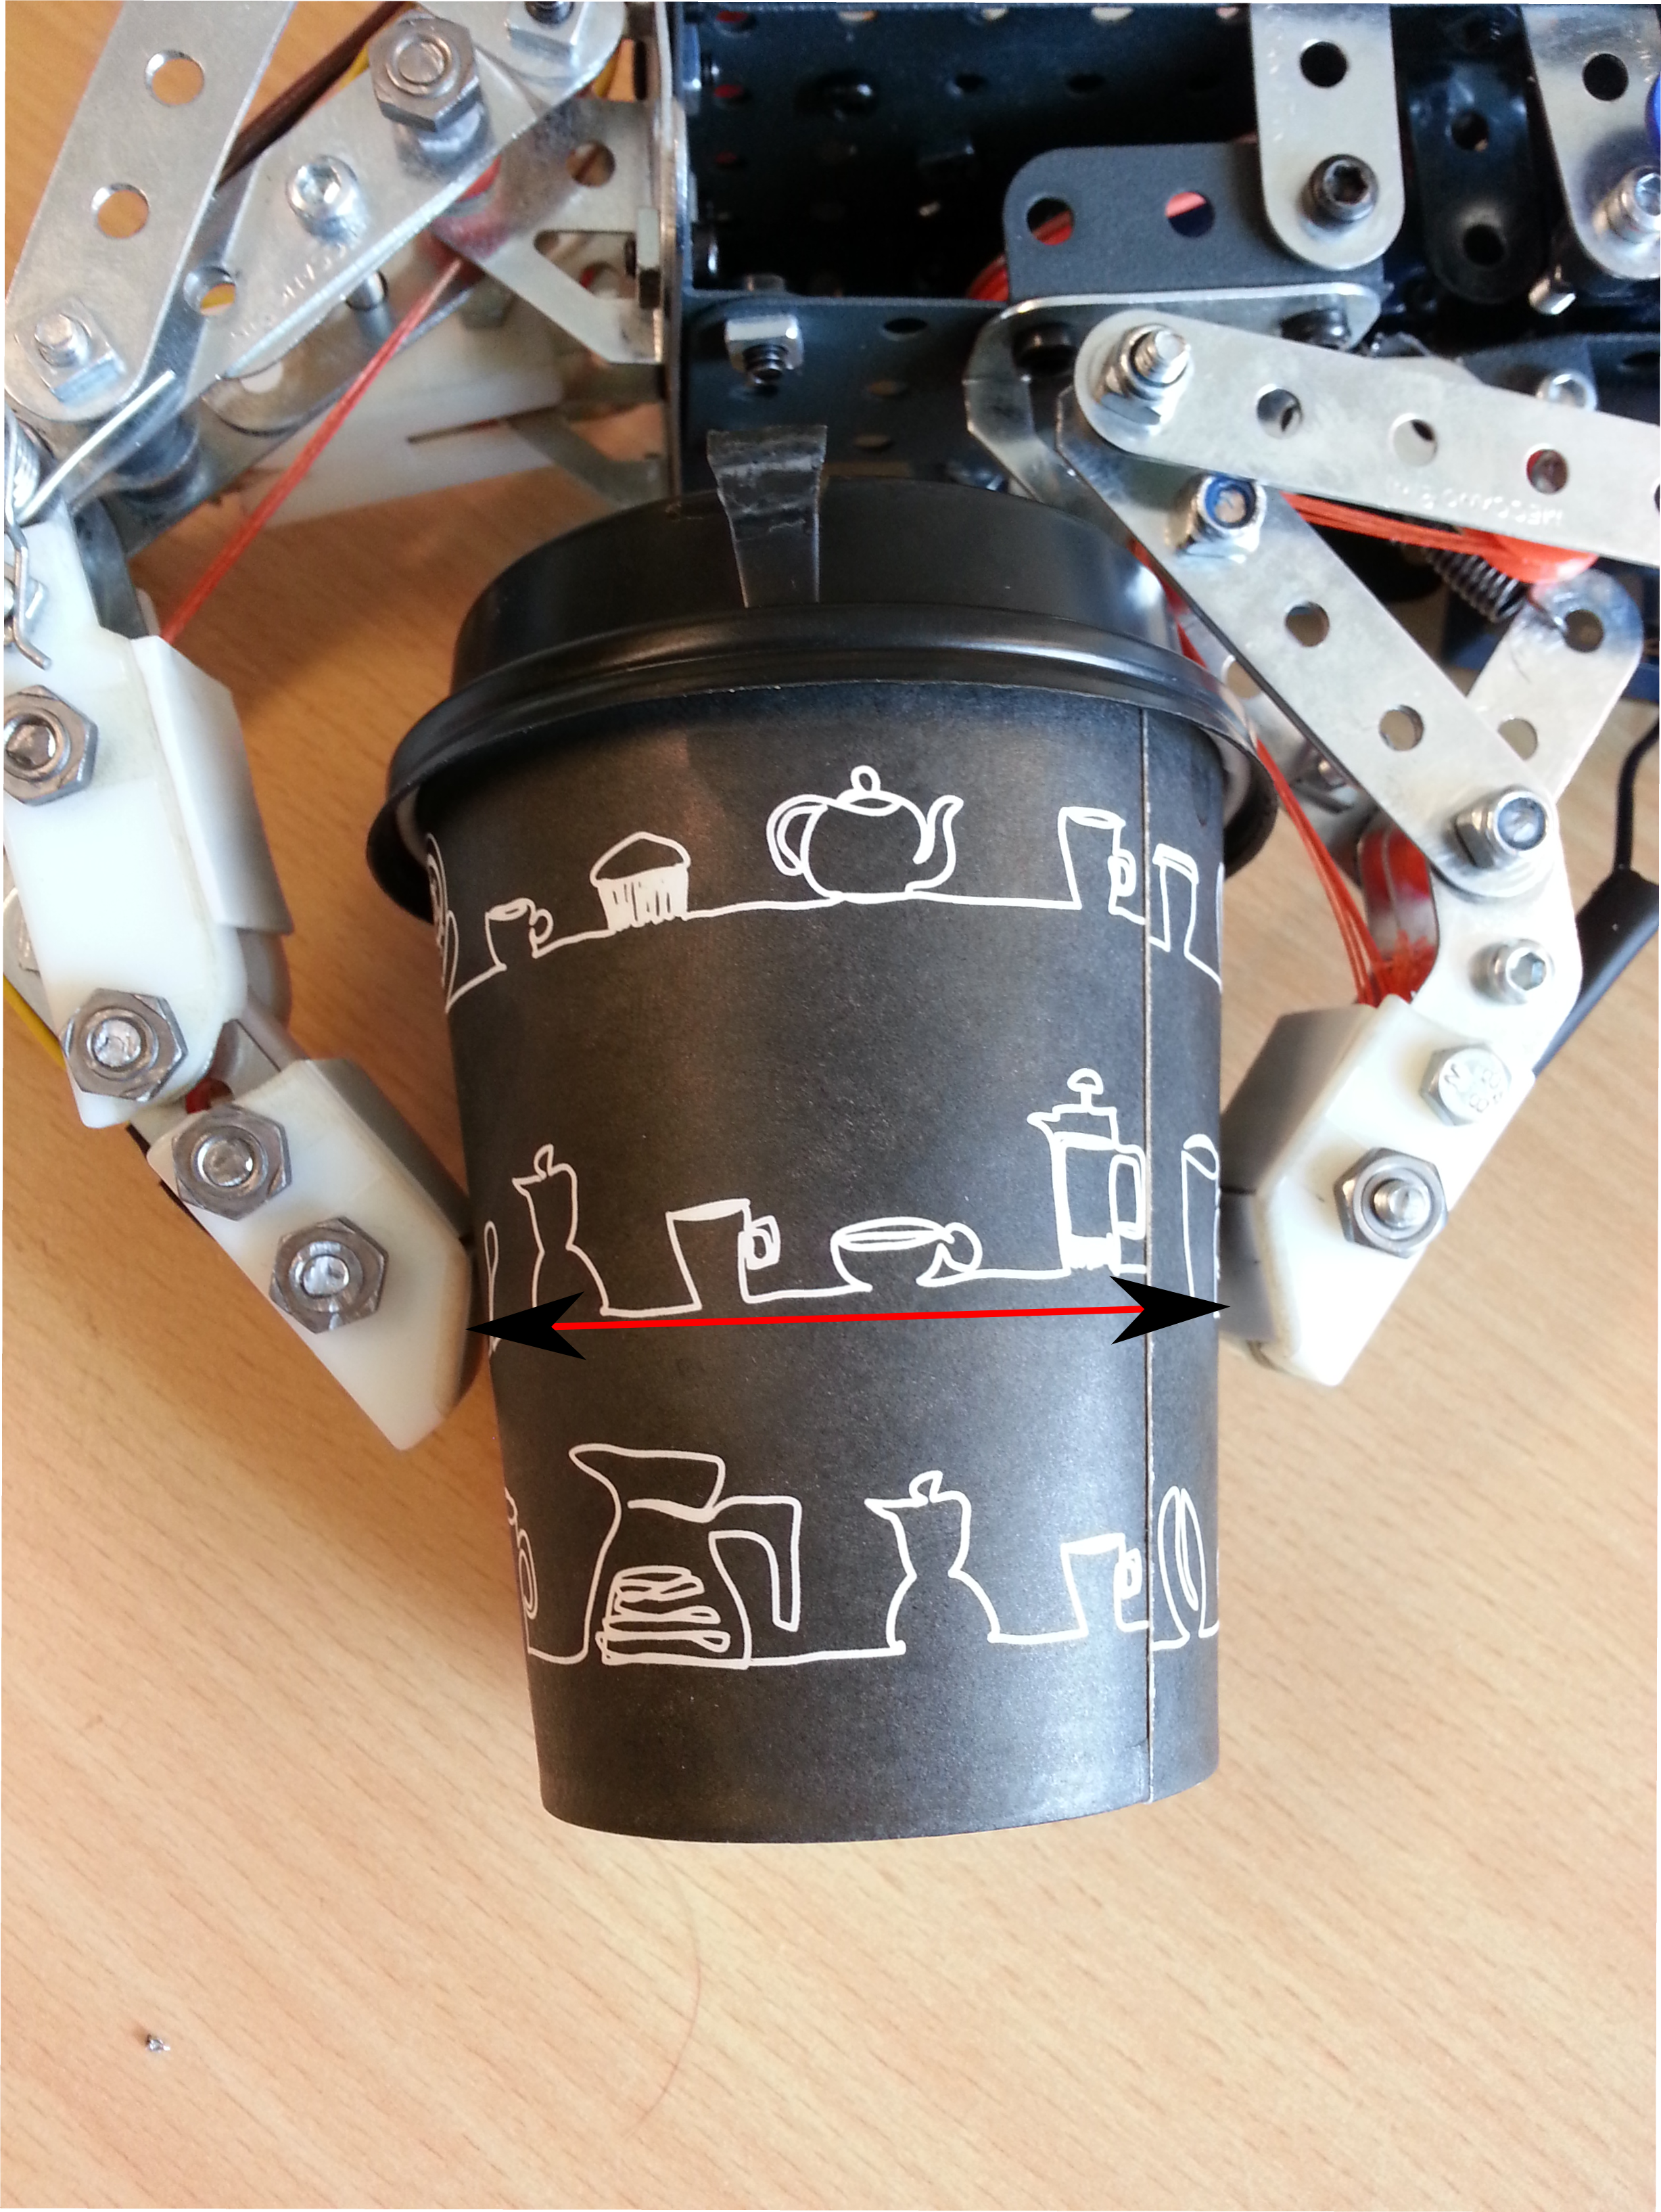
\includegraphics{img/obj_dist}
\caption{Identifiering av objekt.}
\label{fig:objektid}
\end{figure}

För att beräkna avståndet mellan fingertopparna har en matematisk modell av handen tagits fram. Den utgår från servomotorernas önskade vridningsvinklar för att bestämma hur fingrarna är ställda. Då ingen mätning av servomotorernas faktiska läge görs finns endast information om den önskade vinkeln, men då servomotorerna reglerar sig själva kommer de efter en viss tidsfördröjning nå dit, förutsatt att de inte blir behindrade. Denna tidsfördröjning försummas då den är liten vid de små manipulationer av robothanden som görs då användaren försöker gripa ett objekt. Totalt är det fyra servomotorer som inverkar på avståndet mellan fingertopparna.
\begin{figure}[H]
\includegraphics[width=0.5\textwidth]{img/servo/servo_vinklar}
\caption{Samtliga servovinklar för finger 1 och tumme.}
\label{fig:vinklar}
\end{figure}
Modellen baseras på vridningsvinklarna ($\varphi_1$,$\varphi_2$,$\varphi_3$,$\varphi_4$), se figur~\ref{fig:vinklar} som är de servolägen som entydigt bestämmer avståndet mellan fingertopparna. 
\begin{figure}[H]
\includegraphics[width=0.8\textwidth]{img/servo/matlab_modell}
\caption{Matematisk modell över handen plottad i matlab.}
\label{fig:matlabmodell}
\end{figure}
En fullständig matematisk modell av finger 1 och tummen tas fram och demonstreras med hjälp av matlab i figur~\ref{fig:matlabmodell} ovan. Modellen implementeras i robothandens mikrokontroller används för att beräkna avståndet mellan trycksensorerna.  För fullständig beräkningsgång från servovinklar till beräknat avstånd, se appendix~\ref{servoberakningar}.



\section{Begränsning av tryckkraft}
Då robothanden identifierat ett objekt erhålles ett maximalt tillåtet kontakttryck för detta objekt. Om sensorerna registrerar att detta tryck uppnås kommer servomotorerna för det aktuella fingret stoppas, så att högre trycknivå inte uppnås. Så länge användaren håller sin hand sluten kommer robothanden hålla kvar vid det stoppade läget, för att sedan när användaren öppnar sin hand återgår till att följa användarens rörelser igen.